\documentclass{standalone}
\usepackage{tikz}
\usepackage{ctex,siunitx}
\setCJKmainfont{Noto Serif CJK SC}
\usepackage{tkz-euclide}
\usepackage{amsmath}
\usetikzlibrary{patterns, calc,3d,trees}
\usetikzlibrary {decorations.pathmorphing,decorations.pathreplacing,decorations.shapes}
\begin{document}
\small
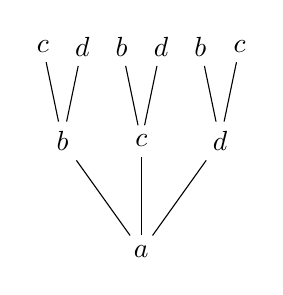
\begin{tikzpicture}
  \node {$a$}
    [grow via three points={
one child at (0,1) and two children at (-.5,1.2) and (.5,1.2)}]
    child { node {$b$}
    [grow via three points={
one child at (0,1) and two children at (-.25,1.2) and (.25,1.2)}]
      child {node {$c$}}
      child {node {$d$}}
    }
    child { node {$c$}
    [grow via three points={
one child at (0,1) and two children at (-.25,1.2) and (.25,1.2)}]
      child {node {$b$}}
      child {node {$d$}}
    }
    child { node {$d$}
    [grow via three points={
one child at (0,1) and two children at (-.25,1.2) and (.25,1.2)}]
      child {node {$b$}}
      child {node {$c$}}
    };
\end{tikzpicture}
\end{document}